\documentclass{article}
\usepackage{amsmath,amssymb}
\usepackage{tikz}
\usetikzlibrary{arrows.meta,positioning,calc,shapes.geometric}
\pagestyle{empty}
\begin{document}
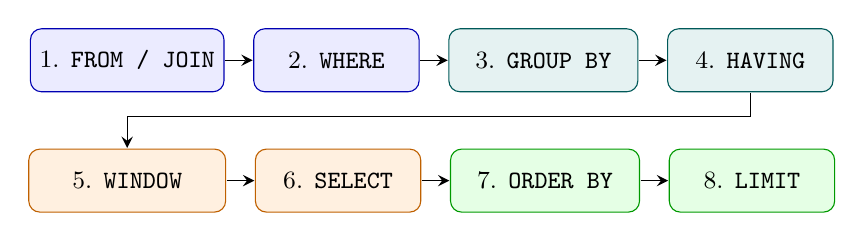
\begin{tikzpicture}
\tikzset{node distance=1.4cm, >=stealth, thick, font=\small}
\node[draw=blue!70!black, fill=blue!8, rounded corners, minimum width=2.4cm, minimum height=0.8cm, align=center] (from) {1. \texttt{FROM / JOIN}};
\node[draw=blue!70!black, fill=blue!8, rounded corners, minimum width=2.1cm, minimum height=0.8cm, align=center, right=0.35cm of from] (where) {2. \texttt{WHERE}};
\node[draw=teal!70!black, fill=teal!10, rounded corners, minimum width=2.4cm, minimum height=0.8cm, align=center, right=0.35cm of where] (group) {3. \texttt{GROUP BY}};
\node[draw=teal!70!black, fill=teal!10, rounded corners, minimum width=2.1cm, minimum height=0.8cm, align=center, right=0.35cm of group] (having) {4. \texttt{HAVING}};
\node[draw=orange!75!black, fill=orange!12, rounded corners, minimum width=2.5cm, minimum height=0.8cm, align=center, below=0.7cm of from] (win) {5. \texttt{WINDOW}};
\node[draw=orange!75!black, fill=orange!12, rounded corners, minimum width=2.1cm, minimum height=0.8cm, align=center, right=0.35cm of win] (sel) {6. \texttt{SELECT}};
\node[draw=green!60!black, fill=green!10, rounded corners, minimum width=2.4cm, minimum height=0.8cm, align=center, right=0.35cm of sel] (ord) {7. \texttt{ORDER BY}};
\node[draw=green!60!black, fill=green!10, rounded corners, minimum width=2.1cm, minimum height=0.8cm, align=center, right=0.35cm of ord] (lim) {8. \texttt{LIMIT}};
\draw[->] (from) -- (where);
\draw[->] (where) -- (group);
\draw[->] (group) -- (having);
\draw[->] (having.south) -- ++(0,-0.3) -| (win.north);
\draw[->] (win) -- (sel);
\draw[->] (sel) -- (ord);
\draw[->] (ord) -- (lim);
\end{tikzpicture}
\end{document}
